\documentclass[tikz]{standalone}
\usepackage[dvipsnames,svgnames,x11names]{xcolor}
\usepackage{tikz}
\usepackage{pgfplots}
\usetikzlibrary{pgfplots.statistics}
\pgfplotsset{compat = 1.12}
\usepackage[
  group-separator={,},
  exponent-product=\cdot,
]{siunitx}
\usepackage{../thesismath}
\begin{document}
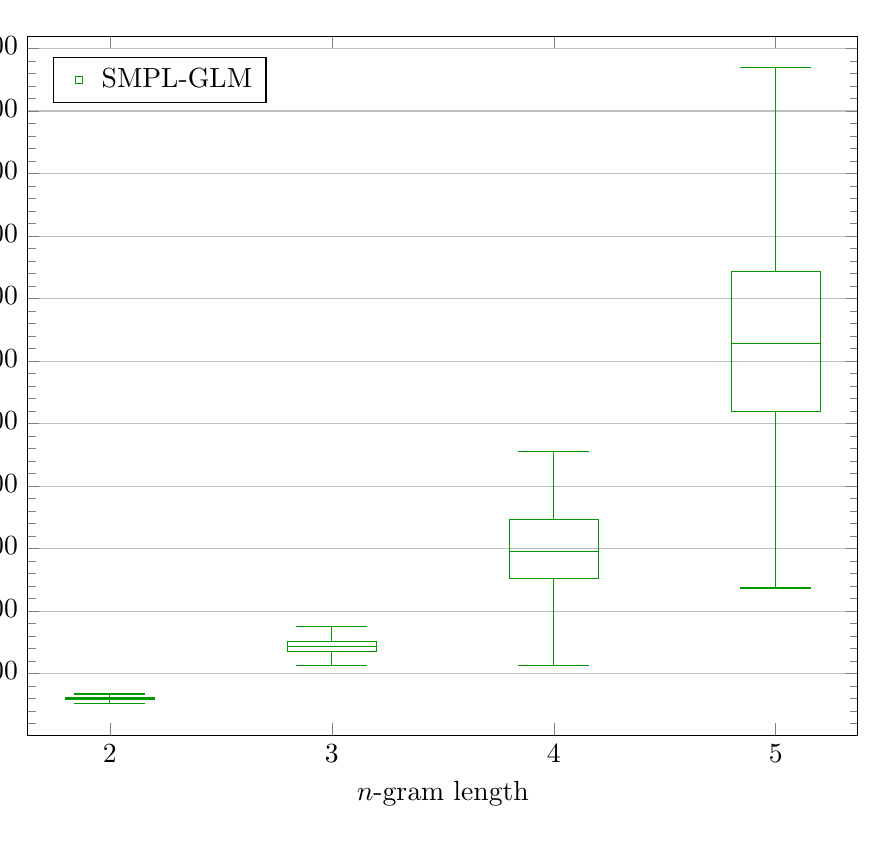
\begin{tikzpicture}[baseline, trim axis left, trim axis right]

\pgfplotscreateplotcyclelist{smpl}{%
  green!60!black,  mark size=1.25, mark=square,\\%
  %blue,  mark size=1.25, mark=square,\\%
  %red,   mark size=1.25, mark=square,\\%
}

\pgfplotsset{
  legend style = {
    legend image code/.code = {
      \draw[only marks]
        plot coordinates {
          (0.3cm,0cm)
        };
      \node at (0.15cm, 0cm) {};
      \node at (0.45cm, 0cm) {};
    },
  },
  boxplot/draw/average/.code = {
    % uncomment to show dotted bars for average:
    %\draw[dashed, /pgfplots/boxplot/every average/.try]
    %  (boxplot box cs:\pgfplotsboxplotvalue{average},0)
    %  --
    %  (boxplot box cs:\pgfplotsboxplotvalue{average},1)
    %  ;
  },
}

\sisetup{exponent-base = 2}
\begin{axis}[
%   title = {Calculation Time per top-$1$ Prediction using $5$-grams},
  xlabel = {$n$-gram length},
  xtick = {2, ..., 5},
  ylabel = {Calcluation Time [\si{\milli\second}]},
  ymin = 1052.826039,
  ymax = 21379.195192,
  scaled x ticks = false,
  scaled y ticks = false,
  minor y tick num = 4,
  ymajorgrids = true,
  boxplot/draw direction = y,
  boxplot = {
    box extend = 0.4,
  },
  cycle list name = smpl,
  enlargelimits = 0.05,
  legend entries = {{SMPL-GLM}},
  legend pos = north west,
  width = \textwidth,
]

% ------------------------------------------------------------------------------

% ngram-2-1k-SMPL-Weighted-Sum-Generalized-Language-Model-1
\addplot+[
  boxplot prepared = {
    draw position = 2,
    lower whisker = 1052.826039,
    lower quartile = 1163.378145,
    median = 1197.428237,
    upper quartile = 1238.655275,
    upper whisker = 1350.590684,
    average = 1204.338189,
  },
] table [row sep = \\, y index = 0] {
  data\\
};

% ------------------------------------------------------------------------------

% ngram-3-1k-SMPL-Weighted-Sum-Generalized-Language-Model-1
\addplot+[
  boxplot prepared = {
    draw position = 3,
    lower whisker = 2272.469670,
    lower quartile = 2700.682233,
    median = 2870.146515,
    upper quartile = 3036.221748,
    upper whisker = 3512.689833,
    average = 2757.968834,
  },
] table [row sep = \\, y index = 0] {
  data\\
};

% ------------------------------------------------------------------------------

% ngram-4-1k-SMPL-Weighted-Sum-Generalized-Language-Model-1
\addplot+[
  boxplot prepared = {
    draw position = 4,
    lower whisker = 2262.708130,
    lower quartile = 5054.943710,
    median = 5923.403096,
    upper quartile = 6929.972684,
    upper whisker = 9121.043219,
    average = 5956.168737,
  },
] table [row sep = \\, y index = 0] {
  data\\
};

% ------------------------------------------------------------------------------

% ngram-5-1k-SMPL-Weighted-Sum-Generalized-Language-Model-1
\addplot+[
  boxplot prepared = {
    draw position = 5,
    lower whisker = 4741.025183,
    lower quartile = 10381.878531,
    median = 12565.672071,
    upper quartile = 14875.880460,
    upper whisker = 21379.195192,
    average = 12622.954410,
  },
] table [row sep = \\, y index = 0] {
  data\\
};

\end{axis}

\end{tikzpicture}
\end{document}
